\documentclass[a4paper,10pt]{article}
\usepackage[utf8]{inputenc}
\usepackage[a4paper,margin=3.5cm]{geometry} %Sets the page geometry
\usepackage{url}
\usepackage{dirtytalk}
\usepackage{graphicx} % Package for \includegraphics
\usepackage{wrapfig} % Figure wrapping
\usepackage[T1]{fontenc} % Output font encoding for international characters
\setlength{\parskip}{1em} % Set space when paragraphs are used
\usepackage{amssymb}
\usepackage{amsmath}
\usepackage{tcolorbox}
\usepackage{mathtools}
\usepackage{tikz}
\usepackage{amsthm}
\usepackage{caption}
\usetikzlibrary{arrows}

% Self Explanatory
\newtheorem{theorem}{Theorem}[section]
\newtheorem{definition}{Definition}[section]
\newtheorem{corollary}{Corollary}[theorem]
\newtheorem{lemma}[theorem]{Lemma}
\newtheorem{exercise}{Exercise}[section]

\theoremstyle{definition} % Set solutions to be bold
\newtheorem*{solution}{Solution}

% Other
\DeclarePairedDelimiter\floor{\lfloor}{\rfloor} %Floor function

% Remove indentation for paragraphs
\setlength{\parindent}{0pt}

% Change footnote numbering to numeric style
\renewcommand{\thefootnote}{\arabic{footnote}}


\begin{document}
    \section{Lecture 01}
    This course deals with \emph{abstract mathematical objects}, which
    are defined by the properties they satisfy.

    \textbf{Properties:} defined by propositions/statements which are either true or false. 
    Here are a few examples of propositions:
    \begin{enumerate}
        \item 7 is a prime number.
        \item All natural numbers are even.
        \item All even numbers greater than 2 can be written as the sum of 2 primes.
    \end{enumerate}

    We shall try to define the natural numbers themselves using the properties 
    they satisfy. Let's start with these 2 axioms:

    \begin{tcolorbox}[colback=blue!10!white, colframe=blue!50!black]
    \begin{enumerate}
        \item $0$ is a natural number. \footnotemark
        \item For every natural number $n$, there exists a natural number $n+1$.
    \end{enumerate}
    \end{tcolorbox}
    \footnotetext{Whether we add 0 or not to the set of natural numbers is simply a 
    matter of convention. For this course, it is convenient to add it to the set.}

    The first axiom tells us that there is a starting number (which we call 0), 
    and the second axiom tells us that for every natural number there is a \emph{next} 
    natural number.

    It might be a bit weird to use the addition symbol in our axioms when we haven't 
    even defined numbers yet. Note that this is just a notation; to make it clear
    we can write $next(n)$ instead of $n+1$ to indicate the next natural number. 
    It's best to think of $next(n)$ as a function which just spits out a new natural
    number for each input $n$.

    \textbf{Predicates: }a statement which involves variables, which can take any value
    in some domain. Think of a predicate $P(x)$ as a function which assign true or 
    false to each value x. For example, $P(x)$ could denote \emph{x is the square of
    an integer}.

    There are 3 ways to make a predicate into a proposition:
    \begin{enumerate}
        \item Substitute a constant for x, for example $P(18)$ is a proposition.
        \item $\exists x \ P(x)$: this proposition is true if there is some object
        $a$ for which $P(a)$ is true.
        \item $\forall x \ P(x)$: this proposition is true if $P(x)$ is true for all
        objects x. 
    \end{enumerate}

    Using this notation, we can precisely write our previous 2 axioms for natural numbers:
    \begin{tcolorbox}[colback=blue!10!white, colframe=blue!50!black]
    \begin{enumerate}
        \item $\exists n \ n = 0$
        \item $\forall n \ \exists m \ (m = next(n))$
    \end{enumerate}
    \end{tcolorbox}

    Let's think more about the second axiom. We need to place more restrictions on this 
    \emph{next} function to get our natural numbers. For example, if we allow $next(0) = 0$, 
    our natural numbers just becomes the set $\{0\}$, and it satisfies the axioms we have so far.
    We could also have $next(0) = 1, next(1) = 0$. So one restriction we could think of to
    avoid this is to keep $next(n) \neq 0$ for all $n$.

    \begin{figure}[ht]
    \centering
    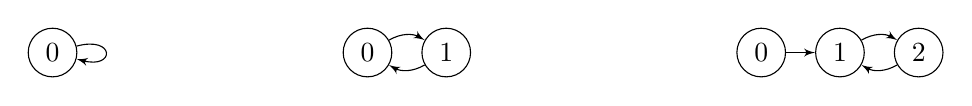
\begin{tikzpicture}
        \tikzset{vertex/.style = {shape=circle,draw,minimum size=1.5em}}
        \tikzset{edge/.style = {->,> = latex'}}
        % vertices
        \node[vertex] (a0) at (0,0) {0};
        \node[vertex] (b0) at (4,0) {0};
        \node[vertex] (b1) at (5,0) {1};
        \node[vertex] (c0) at (9,0) {0};
        \node[vertex] (c1) at (10,0) {1};
        \node[vertex] (c2) at (11,0) {2};
        %edges
        \draw[edge] (a0) to [loop right] ();
        \draw[edge] (b0) to [bend left] (b1);
        \draw[edge] (b1) to [bend left] (b0);
        \draw[edge] (c0) to (c1);
        \draw[edge] (c1) to [bend left] (c2);
        \draw[edge] (c2) to [bend left] (c1);
        
    \end{tikzpicture}

    \caption[Caption for LOF]{Valid number systems\footnotemark\ without any condition
    on \emph{next}}
    \end{figure}
    \footnotetext{It's important to keep in mind what makes one number system different
    from another is how the nodes are linked, it's not about what symbol we keep for each
    node like 0, 1, 2}

    Is this enough? Not really, as we can still think of counterexamples, like
    $next(0) = 1, next(1) = 2, next(2) = 1$. Basically we have ensured that \emph{next}
    doesn't loop back to 0. But we must ensure that it doesn't loop back at all 
    (or even to the same number). How we shall do this is to add the restriction that 
    \emph{next} should not point to a number which has already been mapped to i.e. we make
    it a one-one function. Let's now add these conditions to our axioms:

    \begin{tcolorbox}[colback=blue!10!white, colframe=blue!50!black]
        \begin{enumerate}
            \item $\exists n \ n = 0$
            \item $\forall n \ \exists m \ (m = next(n))$
            \begin{enumerate}
                \item $\forall n \ next(n) \neq 0$
                \item $\forall m \ \forall n \ next(m) = next(n) \implies m = n$
            \end{enumerate}
        \end{enumerate}
    \end{tcolorbox}

    \begin{figure}[ht]
    \centering
    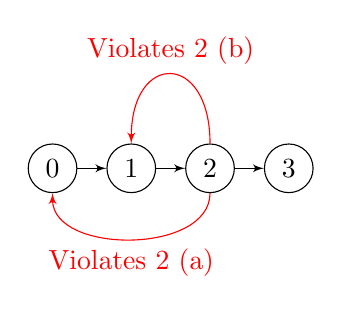
\begin{tikzpicture}
        \tikzset{vertex/.style = {shape=circle,draw,minimum size=1.5em}}
        \tikzset{edge/.style = {->,> = latex'}}
        % vertices
        \node[vertex] (0) at (0,0) {0};
        \node[vertex] (1) at (1,0) {1};
        \node[vertex] (2) at (2,0) {2};
        \node[vertex] (3) at (3,0) {3};
        %edges
        \draw[edge] (0) to (1);
        \draw[edge] (1) to (2);
        \draw[edge] (2) to (3);
        \draw[red, edge] (2) to [in=90, out=90, looseness=3] node[midway, above] {Violates 2 (b)} (1);
        \draw[red, edge] (2) to [in=270, out=270, looseness=1] node[midway, below] {Violates 2 (a)} (0);
    \end{tikzpicture}
    \caption{Diagrammatic explanation of why \emph{next} always points to a new number}
    \end{figure}

    It turns out our axioms are still not complete. We have ensured that \emph{next}
    always points to a new number, but we haven't really ensured that every natural
    number can be formed by applying \emph{next} to 0 a finite number of times. 
    Here are some counterexamples:
    \begin{enumerate}
        \item $\left\{0, \frac{1}{3}, \frac{2}{3}, \dots\right\}$ where $next(n) = n+1$ 
        \item $[0, \infty)$ where $next(n) = n+1$
    \end{enumerate}
    
    By repeatedly applying \emph{next} to our growing chain, we should end up 
    with the set of all natural numbers. A neat way of stating this is to just
    keep an axiom that induction itself works i.e. if a statement is true for 
    $0, next(0), next(next(0)), \dots$ it must be true for all natural numbers.
    So here is our final set of axioms, which does lead only to our natural numbers:

    \begin{tcolorbox}[colback=blue!10!white, colframe=blue!50!black]
        \begin{enumerate}
            \item $\exists n \ n = 0$
            \item $\forall n \ \exists m \ (m = next(n))$
            \begin{enumerate}
                \item $\forall n \ next(n) \neq 0$
                \item $\forall m \ \forall n \ next(m) = next(n) \implies m = n$
            \end{enumerate}
            \item $[P(0)] \wedge [\forall n \ \{P(n) \implies P(next(n))\}] \implies [\forall n \ P(n)]$
        \end{enumerate}
    \end{tcolorbox}

    \begin{exercise}
        Prove that $\forall n \ next(n) \neq n$. Can we have this statement instead of 
        2 (b) to define natural numbers?
    \end{exercise}
    \begin{solution}
        Proof by induction \\
        Define $P(n)$ to be $\ next(n) \neq n$. $P(0)$ is true from 2 (a). \\
        Also, $next(n) \neq n \implies next(next(n)) \neq next(n)$ as \emph{next} is one-
        one (or contrapositive of 2 (b)). This is basically $P(n) \implies P(next(n))$. \\
        From this we conclude $P(n)$ i.e. $next(n) \neq n$ for all $n$. \\
        This can't be used instead of 2 (b). Counterexample: $next(0) = 1, next(1) = 2, next(2) = 1$.
    \end{solution}

    \begin{exercise}
        Instead of keeping induction as an axiom, we could ensure that there are no other
        starting points for a chain other than 0. This might ensure that all numbers are
        part of the chain starting from 0. 

        Can we replace axiom 3 with the following: \\ 
        $\forall n \ n \neq 0 \iff \exists m \ next(m) = n$
    \end{exercise}
    \begin{solution}
        No, we have a counterexample, take the set \\ 
        $\{0, 1, 2, \dots\} \cup \{\dots, -1.5, -0.5, 0.5, 1.5, \dots\}$ where $next(n)$ is the standard $n+1$. \\
        It satisfies the new set of 3 axioms but aren't equivalent to natural numbers.
    \end{solution}

    \begin{exercise}
        Is there a more concrete way to show that from axiom 3 that all natural numbers
        can be obtained composing $next$ to 0 a finite (including 0) number of times?
    \end{exercise}
    \begin{solution}
        Let $P(n)$ denote $n$ obtained composing \emph(next) to 0 a finite (including 0) 
        number of times. $P(0)$ is obviously true. It's also clear that $P(n) \implies P(next(n))$,
        as if $n$ can be written as $next(next(\dots(next(0))\dots))$, $next(n)$ can also be written
        that way by just composing one more \emph{next} to the expression. 
        This completes our proof.
    \end{solution}

\end{document}
